\section{Try Resource}
O visitor responsável por detectar a adoção desta \textit{feature} pesquisou por padrões como o código abaixo onde não foi pesquisado oportunidades de \textit{refactoring} mas sim onde esta característica estava sendo adotada.
\begin{lstlisting}
static String readFirstLineFromFile(String path) throws IOException {
	try (BufferedReader br = new BufferedReader(new FileReader(path))) {
		return br.readLine();
	}
}
\end{lstlisting}

Com o advento do Java 7 foi introduzido o \textit{Try with Resource} onde um \textit{resource} é um objeto que pode ser fechado antes do programa ser encerrado. Com isso promoveu uma maior autonomia e flexibilidade ao programador. Foi encontrado no total 284321 \textit{trys} nos quais  esta \textit{feature} totaliza 1.8\%, ou seja, 5186 casos. Conforme exibido na figura: ~\ref{fig:Try with Resource} exibe a distribuição desta \textit{feature} entre os projetos onde pode-se constatar que somente 4 projetos fizera a adoção. Com exceção do projeto \textit{Jetty} que totaliza 87\% dos casos os demais projetos não aderiram de forma massiva esta caracterísitica.


\begin{figure}[h]
	\center
	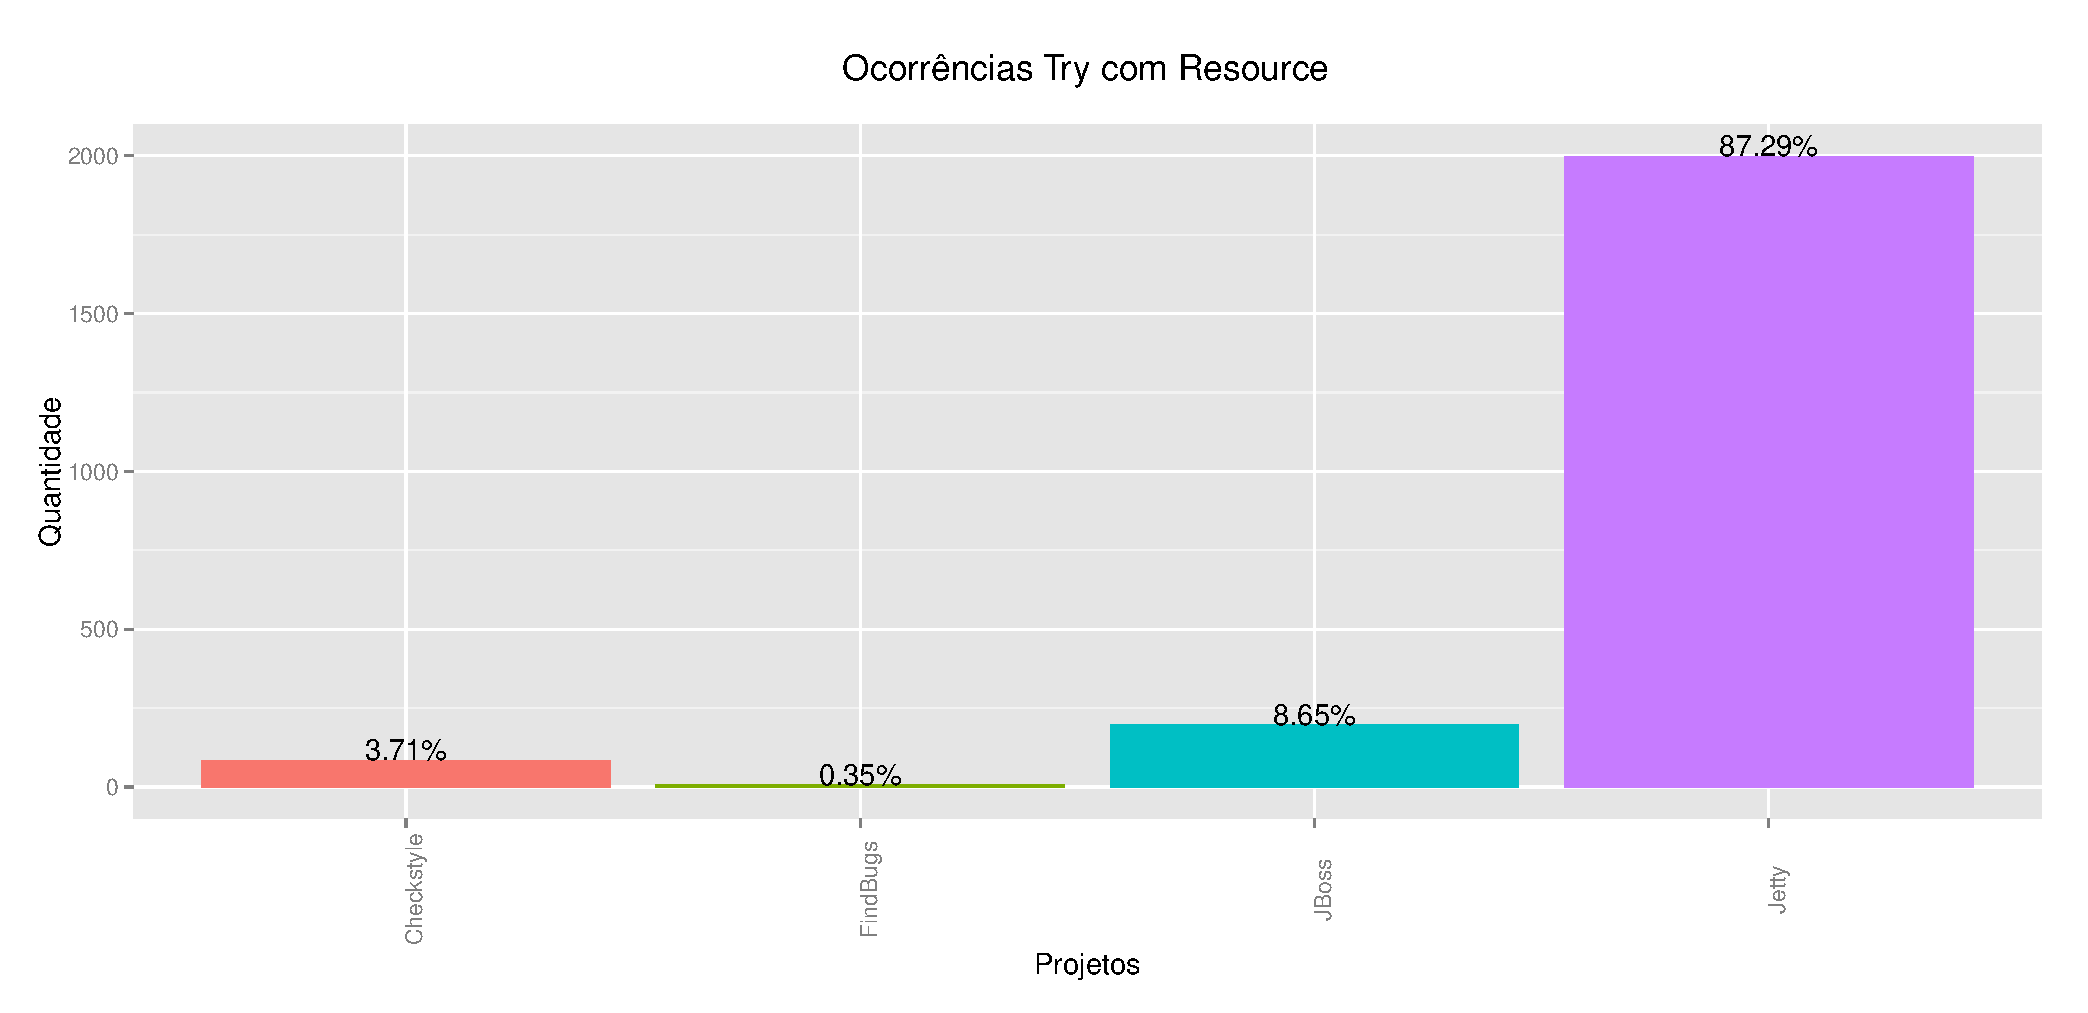
\includegraphics[scale=0.5]{Imagens/ocorrenciasTryResource}
	\label{fig:Try with Resource}
	\caption{Oportunidades de \textit{Try with Resource} nos projetos.}
\end{figure}


